\subsection{Análise mensal}
Foi realizada uma agregação mensal a fim de visualizar as tendências das variáveis do sistema estudado ao longo do ano. Para isso, foi gerada uma tabela com um resumo das médias dos tempos de espera, serviço e de tempo entre chegadas das ligações mês a mês.\\
A partir disso, foi possível calcular a porcentagem de falhas ("\%\_failure") com base na divisão do número total de ligações que demoraram mais de 60 segundos para serem atendidas pelo total de ligações atendidas em cada mês.\\
A partir da Figura \ref*{fig: tmes} é possível visualizar alguns dados relevantes e transformar a base de dados com filtro mês a mês em informações capazes de nos demonstrar o comportamento do processo de atendimento nos quesitos tempo de espera médio, duração média do atendimento, média do tempo entre as chegadas, média do número de ligações recebidas e também a porcentagem de falhas.  

\begin{figure}[H]
    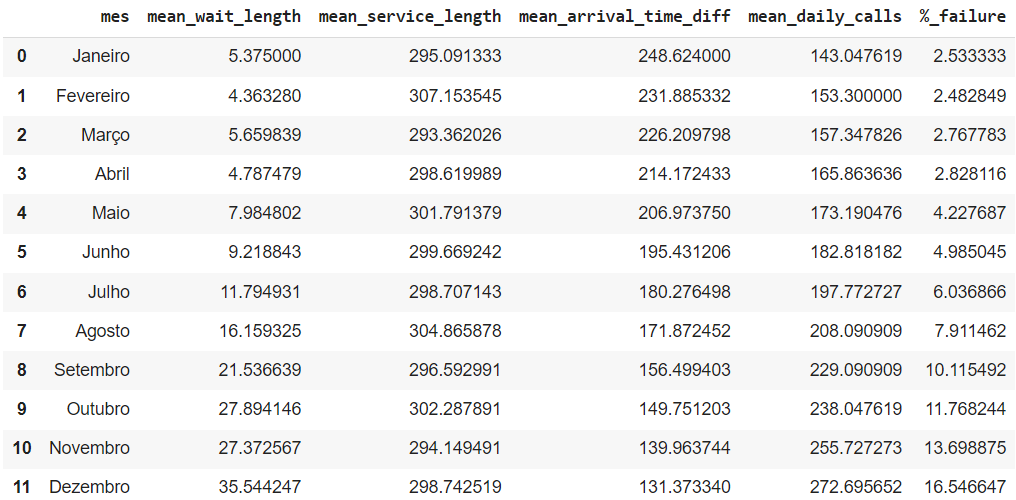
\includegraphics[scale=0.75]{analise-de-dados/mensal/tabmens.png}
    \caption{Tabela de resumo das médias dos tempos de espera, serviço e de chegada de ligações mês a mês}
    \label{fig: tmes}
\end{figure}

Realizando uma análise de cada uma das variáveis do sistema, apoiando-se nos testes de hipótese realizados anteriormente, é possível obter as seguintes conclusões a respeito dessas variáveis:
\begin{itemize}
    \item Tempo de espera: aumenta mês a mês;
    \item Média do tempo de serviço: relativamente constantes;
    \item Tempo entre chegadas: diminui mensalmente;
    \item Número de ligações: aumenta mensalmente;
    \item Percentual de falhas: aumenta mês a mês. A partir de setembro de 2021, a tolerância de 10\% que foi estipulada pelo
     gerente é superada.\\
\end{itemize}

Portanto, o percentual de falhas, aqui definido como o percentual de chamadas que demoram mais de 60 segundos para serem atendidas, aumenta mês a mês, ultrapassando, a partir de setembro de 2021,
a tolerância de 10\% necessária para cumprir a meta de desempenho de 90\% das chamadas atendidas em até 1 minuto.